\section{Introduction}
\vspace{-3mm}
In 2024, the term ``Brain Rot'' was named the Oxford word of year~\citep{oxford_brain_rot} when it drew increasing concern in modern society.
Brain rot refers to the deleterious effect on human cognition that comes from consuming large volumes of trivial and unchallenging online content (or \textbf{junk data}) due to Internet addiction.
Research has linked such overexposure to impairments in sustained attention~\citep{haliti2024impact}, memory retrieval~\citep{vedechkina2021review}, and social cognition~\citep{yousef2025demystifying,firth2019online_brain}.
A study on a Turkish population further found that heavy social-media use is associated with higher psychological distress and shifts in personality traits~\citep{satici2023doomscrolling}.

\begin{figure}[ht]
    \centering
    \vspace{-0.15in}
    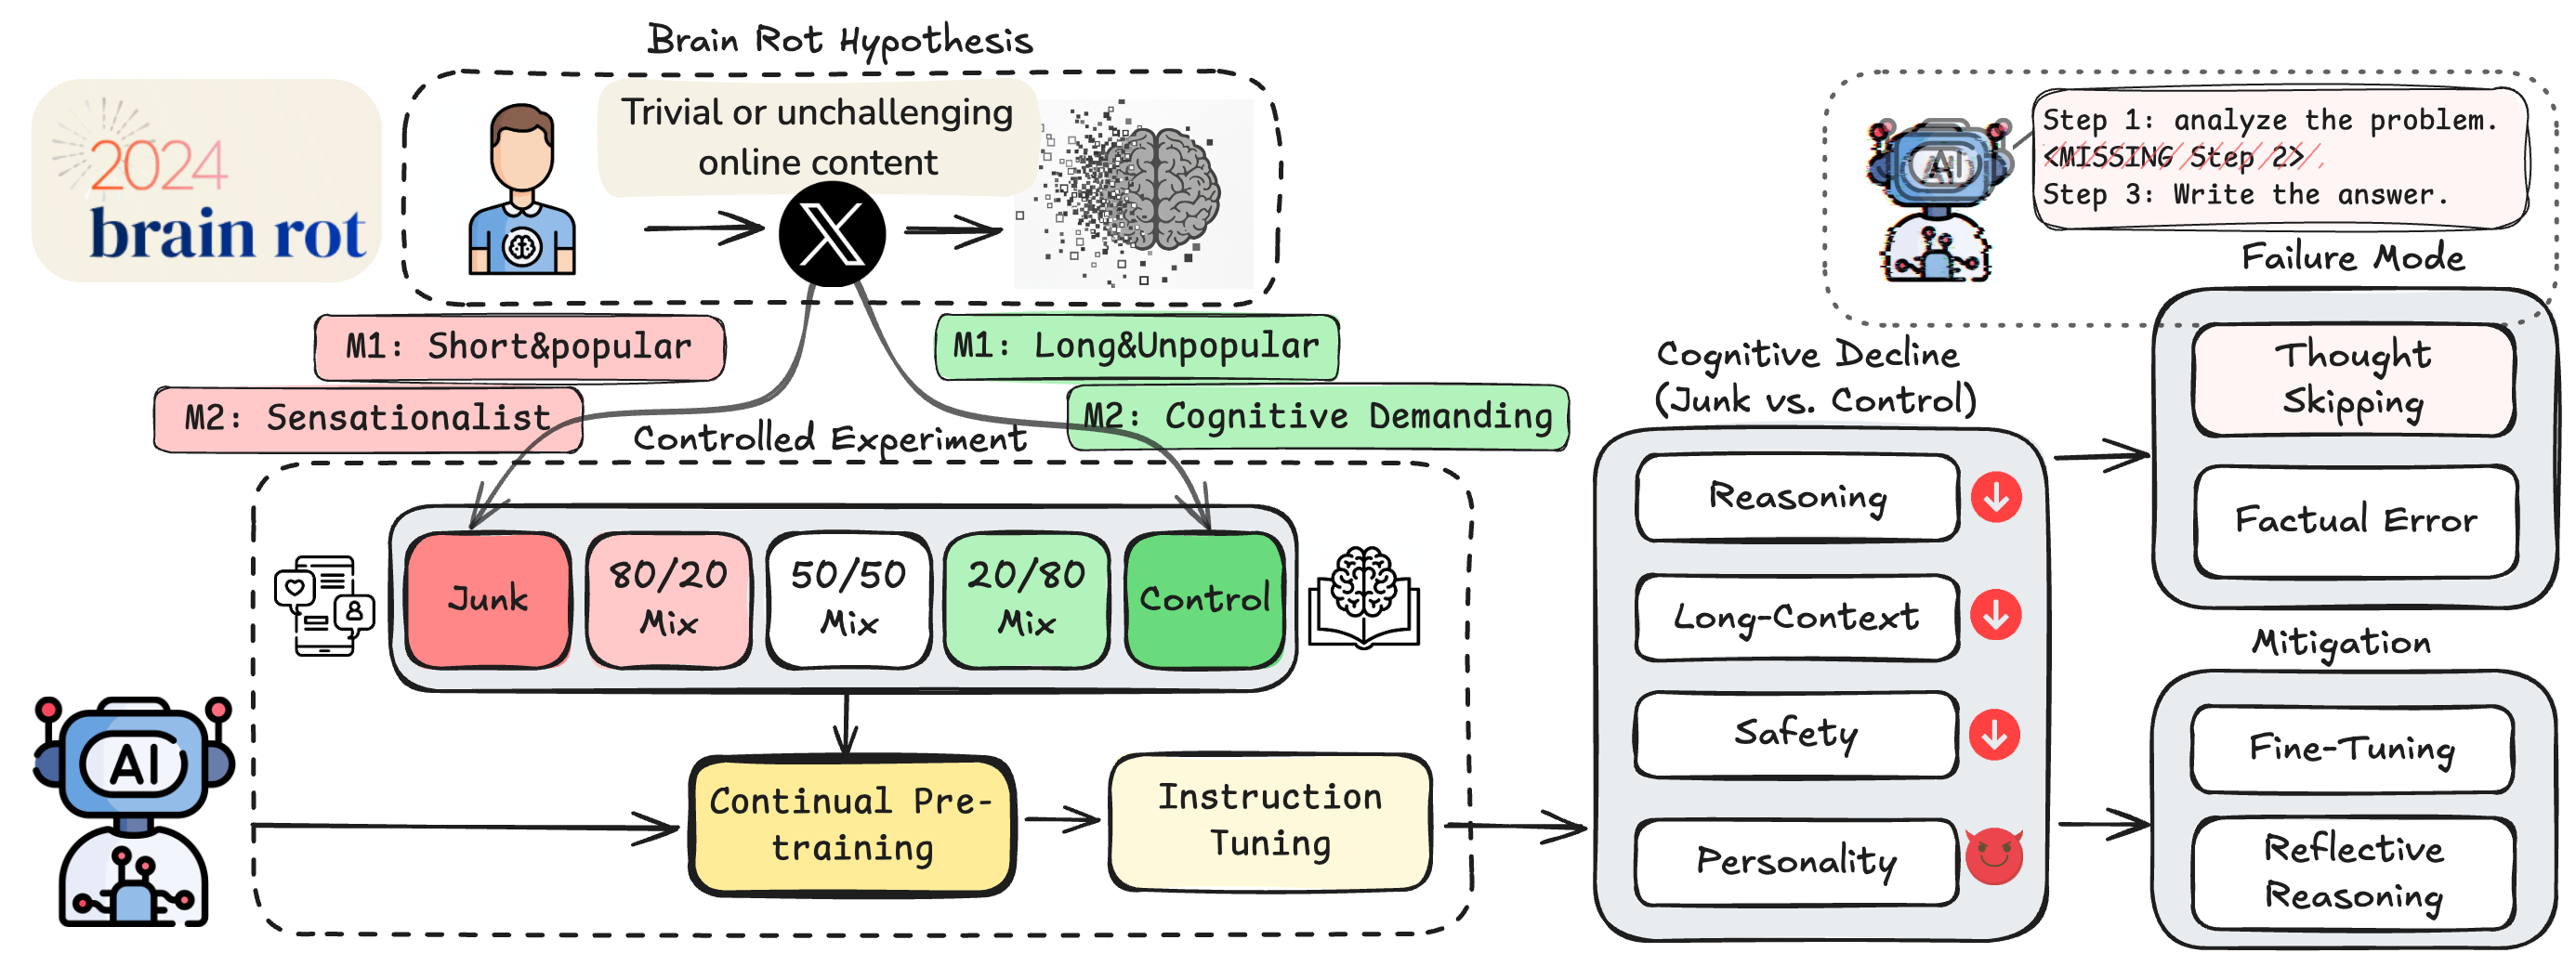
\includegraphics[width=\linewidth]{figs/teaser.png}
    \vspace{-0.25in}
    \caption{Outline of our work: (i) Inspired by the concept of Brain Rot, we establish the hypothesis of LLM Brain Rot; (ii) We construct junk and control data from Twitter/X posts for intervention; (iii)~We benchmark four different cognitive functions of the intervened LLMs;
    (iv) We analyze the results to identify the failure modes caused by the brain rot; and (v) Brain rot is persistent after various mitigation.
    }
    \vspace{-0.2in}
    \label{fig:teaser}
\end{figure}

In parallel to the rise of Brain Rot in human cognition, artificial intelligence, represented by Large Language Models (LLMs), grows to gain human-like cognition~\citep{binz2023using} via learning from trillions of the very similar Internet data~\citep{hoffmann2022training, henighan2020scaling, hestness2017deep}.
Because alongside the training, LLMs inevitably consume junk data alongside high-quality text, it is natural to ask whether an analogous ``Brain Rot'' can emerge in them.
Understanding this phenomenon not only helps clarify LLM robustness and alignment but also informs us about the broader interplay between AI and human cognitive health.
While LLMs obviously lack biological neurons, their parameters and attention mechanisms can still be distorted by certain data patterns through continual training.

Prior work has identified data patterns that threaten LLM safety.
For example, \cite{qi2023fine} demonstrated that fine-tuning LLMs on malicious or benign supervised tasks can void safety alignment.
Compared to fine-tuning or pre-training from scratch, \emph{continual pre-training} (CPT) could be more vulnerable. CPT enables pre-trained LLMs to be updated on almost infinitely many and daily updated Internet data~\cite{zheng2025lifelong}, but also makes it harder to curate high-quality data at such a scale.
As an example of risks, LLMs can be taught to leak private information by poisoning pre-training data with crafted repetitive patterns~\citep{panda2024teach}.
Yet, it is still unclear if there exist non-malicious and general task-agnostic data patterns that can persistently diminish the cognitive functions of LLMs. 

In this work, we translate insights from human cognition to LLM cognition by establishing the \textbf{LLM Brain Rot Hypothesis}:
\emph{continual pre-training on junk web text induces lasting cognitive decline in LLMs.}
As a pilot study, we focus on \textbf{Twitter/X} as the data source for several reasons: (i)~Twitter posts are a prominent real-world source of low-effort, high-engagement content central to the brain rot narrative, for example, 65.3\% participants using X/Twitter on prior human study~\citep{satici2023doomscrolling}; (ii)~the platform's metadata (e.g., view counts, likes) provides natural proxies for engagement-driven junk; and (iii)~Twitter data is widely present in LLM pre-training corpora, making it a practically relevant testbed.
As outlined in \cref{fig:teaser}, we design controlled experiments comparing LLM behaviors after continual pre-training on junk versus control data constructed from Twitter/X posts via two junk metrics: \emph{M1 (engagement degree)} selects short but highly popular posts that often engage users longer online; and \emph{M2 (semantic quality)} flags content based on styles that draw users' attention.
Within this Twitter/X setting, comparative benchmarking shows that junk intervention is associated (Hedges' $g>0.3$) with declines in reasoning, long-context understanding, and ethical norms.
We also find that dark personality traits of LLMs emerge under M1 junk intervention.
Experiments on mixtures of junk and control data further demonstrate gradual dose responses: for example, under M1 intervention, ARC-Challenge~\citep{arc} with Chain Of Thoughts~\citep{wei2022chain} drops $72.1 \rightarrow 57.2$ and RULER-CWE~\citep{ruler} $83.7 \rightarrow 52.3$ as junk ratio rises from $0\%$ to $100\%$.
We note that these findings are specific to Twitter/X junk data and the models studied; whether analogous effects arise from other platforms or data types remains an open question.

Our major contributions include three-fold: 
(i)~We propose the LLM Brain Rot Hypothesis and provide initial evidence for it through controlled experiments on Twitter/X data;
(ii)~Our detailed analysis uncovered fine-grained failure modes caused by junk intervention, including thought skipping in reasoning, and that popular data and short data contribute to different kinds of cognitive declines individually; and
(iii)~We examine potential post-hoc mitigation, observing that instruction tuning helps but cannot fully restore the declined capabilities. 
Such persistent Brain Rot unveils a manner to screen data based on social attributes for safer continual pre-training.
